\chapter{Resultados Experimentales}
\section{Resultados Experimentos}
En este apartado se comentarán los resultados obtenidos por los modelos generados como ensamble de Procesos Gaussianos sobre los diferentes folds de test.

\subsection{Núcleo Gaussiano}
\subsubsection{Fold 1}

\begin{figure}[H]
	\centering
	\subfigure{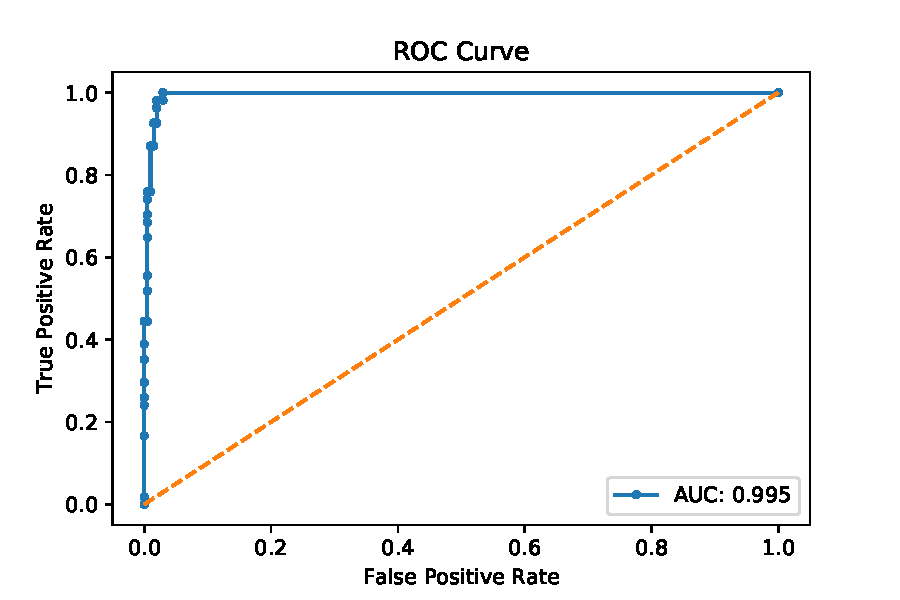
\includegraphics[width=60mm]{imagenes/p1_roc_gpflow}}
	\subfigure{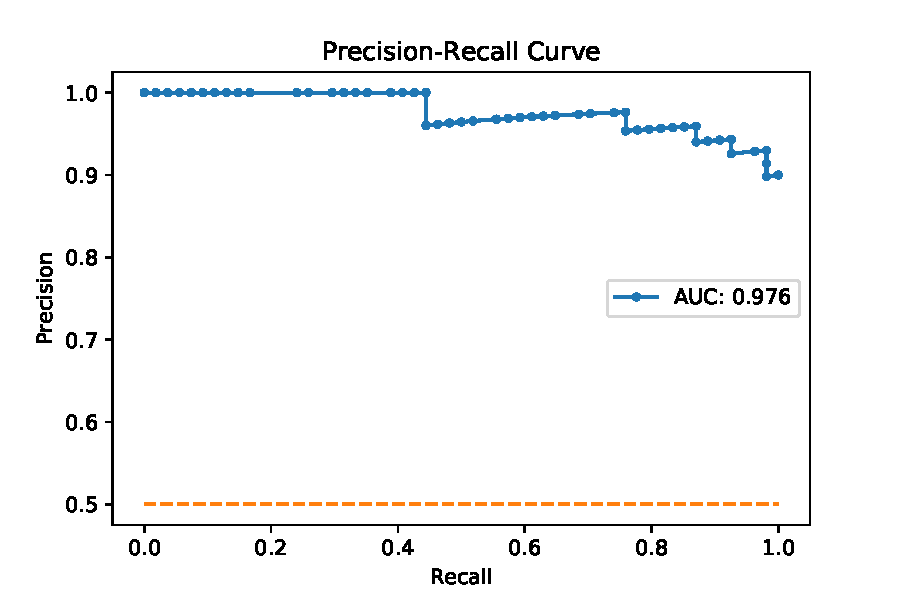
\includegraphics[width=60mm]{imagenes/p1_curve_gpflow}}
	\caption{Curva Roc y Curva Precision-Recall Fold 1 kernel radial}
	\label{fig:resultados1}
\end{figure}

\newpage

\begin{figure}[H]
	\centering
	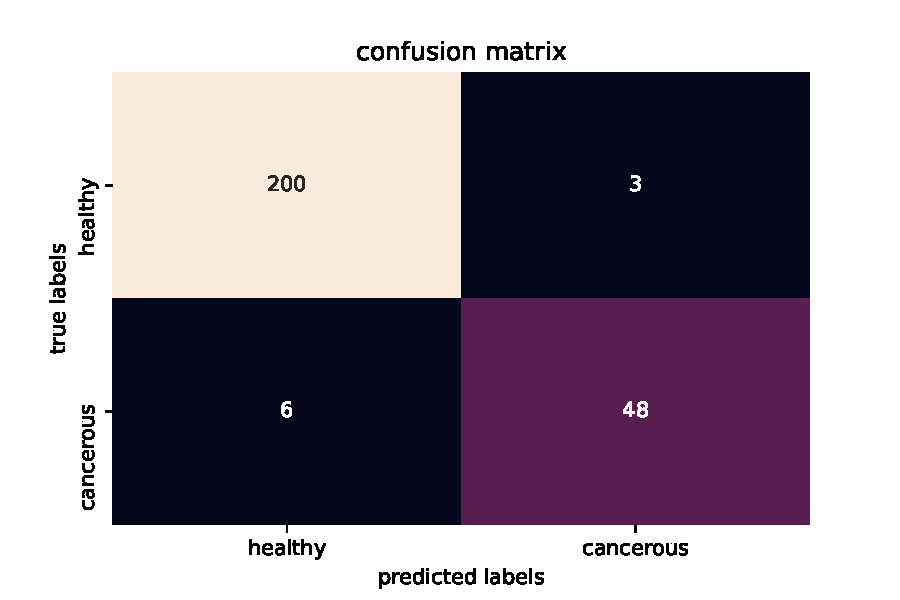
\includegraphics[width=90mm]{imagenes/confusion_mat1_gpflow}
	\caption{Matriz de confusión para Fold 1 kernel radial}
	\label{fig:conf1}
\end{figure}

\begin{table}[H]
	\centering
	\begin{tabular}{lllll}
		\textbf{acc} & \textbf{precision} & \textbf{specificity} & \textbf{recall} & \textbf{f1-score} \\
		0.964981     & 0.941176           & 0.985222             & 0.888889        & 0.914286         \\
	\end{tabular}
	\caption{Resultados obtenidos Fold 1 kernel radial}
	\label{table:1}
\end{table}


Para este fold se obtienen buenos resultados, obteniendo buenos resultados en \textit{Accuracy} y \textit{F1-score}. Si nos fijamos en la \textit{curva ROC} podemos ver que se obtienen muy buenos resultados, obteniendo un valor de \textit{AUC} del 99.5\%, con este valor tan alto podemos decir que está clasificando bastante bien ambas clases. La \textit{curva Precision-Recall} también obtiene buenos resultados, obteniendo un buen valor para su \textit{AUC} también; por lo que se puede ver, se puede ver que hay un buen equilibrio entre \textit{Falsos Positivos} y \textit{Falsos Negativos}, siendo el número de \textit{Falsos Negativos} algo mayor que los \textit{Falsos Positivos}. Si nos fijamos en la matriz de confusión se puede ver que los resultados de las curvas son correctos, viendo que este modelo solamente ha fallado en 9 casos de 257 instancias que tiene este fold; aún siendo buenos resultados, sería mejor que el número de Falsos Positivos fuera mayor que el de \textit{Falsos Negativos}, ya clasificar una imagen como cancerosa aunque después no lo sea a que clasificar una imagen como sana y que sí lo sea por las consecuencias que esto puede tener para un paciente en un caso real.

\subsubsection{Fold 2}

\begin{figure}[H]
	\centering
	\subfigure{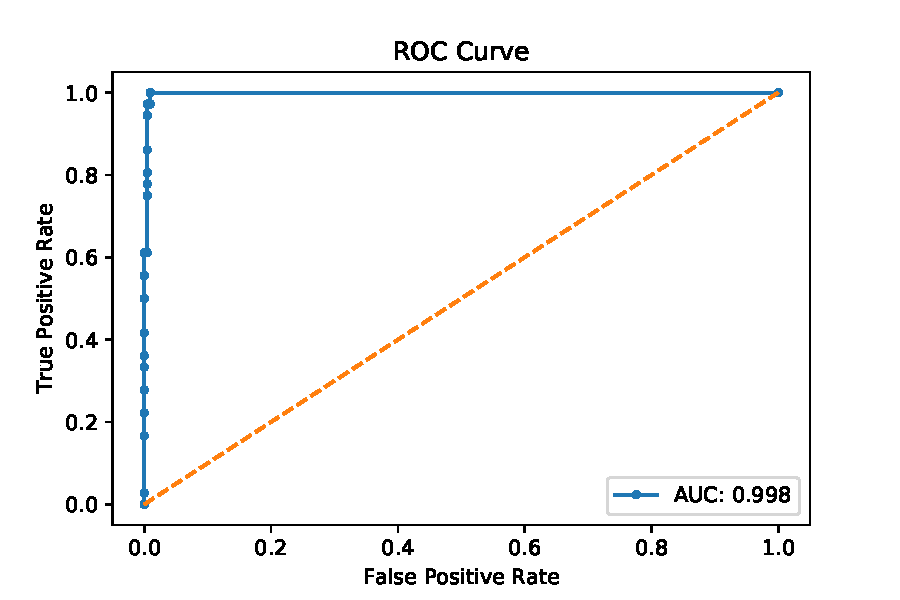
\includegraphics[width=60mm]{imagenes/p2_roc_gpflow}}
	\subfigure{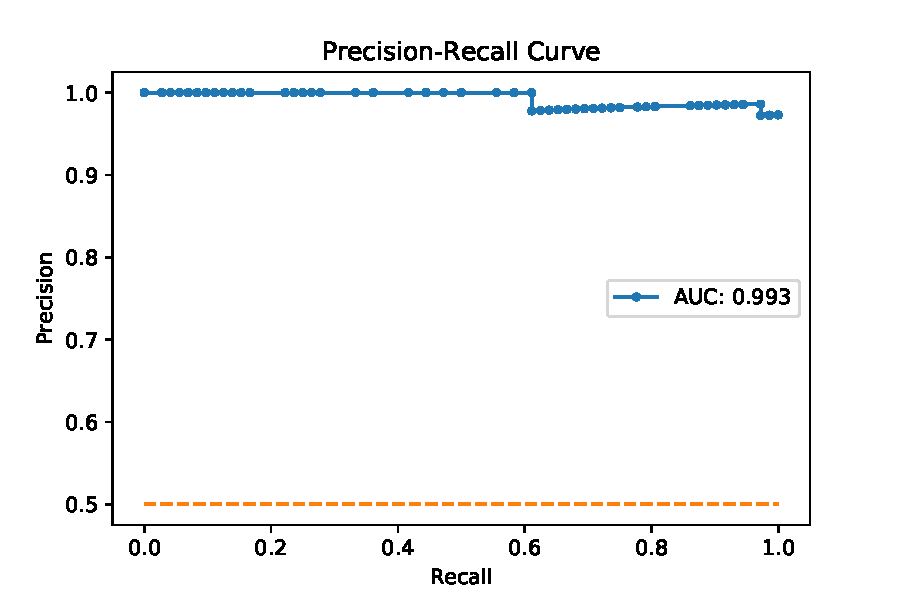
\includegraphics[width=60mm]{imagenes/p2_curve_gpflow}}
	\caption{Curva Roc y Curva Precision-Recall Fold 2 kernel radial}
	\label{fig:resultados2}
\end{figure}

\begin{figure}[H]
	\centering
	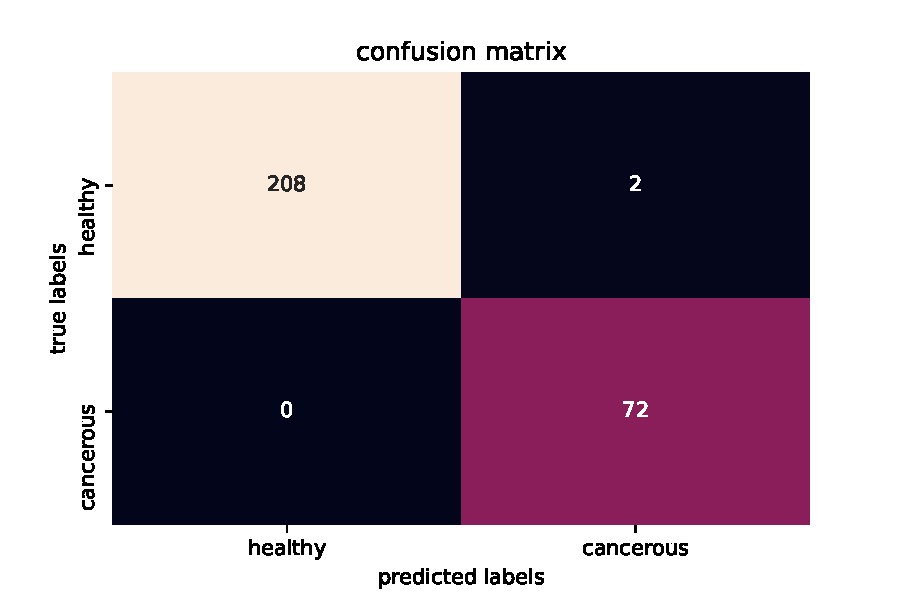
\includegraphics[width=90mm]{imagenes/confusion_mat2_gpflow}
	\caption{Matriz de confusión para Fold 2 kernel radial}
	\label{fig:conf2}
\end{figure}

\begin{table}[H]
	\centering
	\begin{tabular}{lllll}
		\textbf{acc} & \textbf{precision} & \textbf{specificity} & \textbf{recall} & \textbf{f1-score} \\
		0.992908     & 0.972973           & 0.990476             & 1.000000        & 0.986301         \\      
	\end{tabular}
	\caption{Resultados obtenidos Fold 2 kernel radial}
	\label{table:2}
\end{table}

Para este segundo modelo podemos ver mejores resultados todavía que para el modelo anterior, si nos fijamos en las curvas los valores de sus \textit{AUC} son casi 1. Si nos fijamos en las medidas o en la tabla podemos ver que los resultados de la predicción son casi perfectas también, viendo que todas ellas son mayores que el 97\%. Si nos fijamos en la matriz de confusión podemos ver que el clasificador no ha predicho ningún \textit{Falso Negativo}, por lo que este modelo ha conseguido diferenciar mejor entre las imágenes con tejido canceroso y tejido sano y por lo tanto es un mejor modelo que el anterior.

\subsubsection{Fold 3}

\begin{figure}[H]
	\centering
	\subfigure{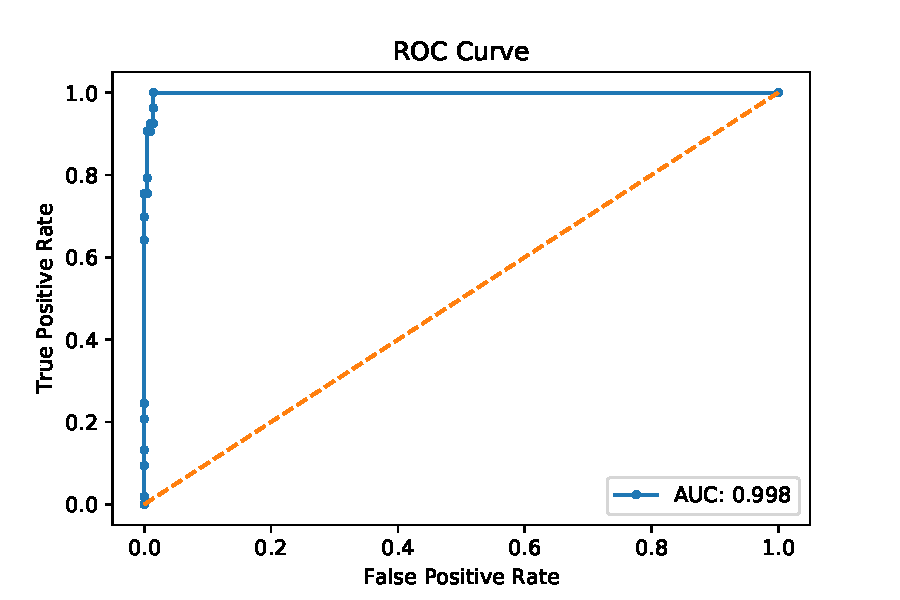
\includegraphics[width=60mm]{imagenes/p3_roc_gpflow}}
	\subfigure{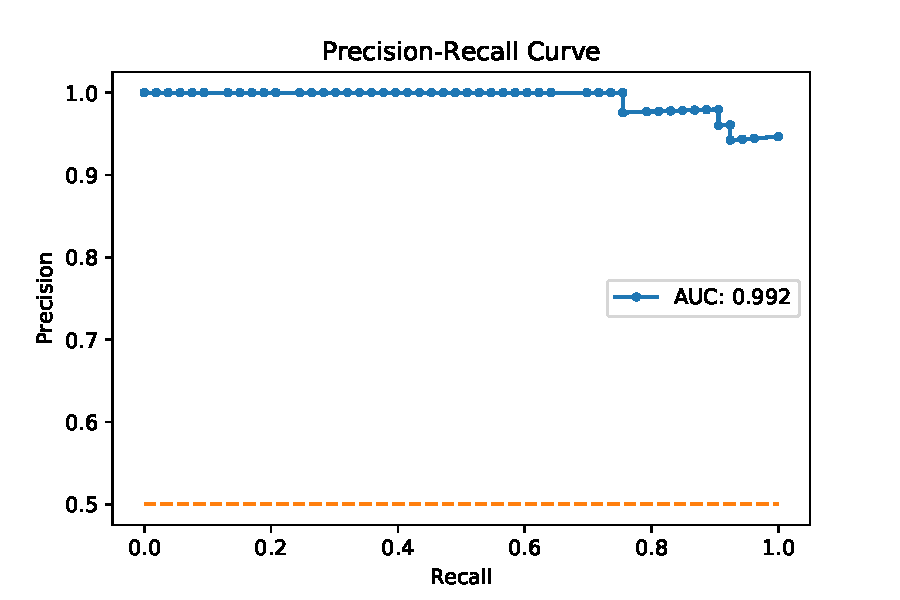
\includegraphics[width=60mm]{imagenes/p3_curve_gpflow}}
	\caption{Curva Roc y Curva Precision-Recall Fold 3 kernel radial}
	\label{fig:resultados3}
\end{figure}

\begin{figure}[H]
	\centering
	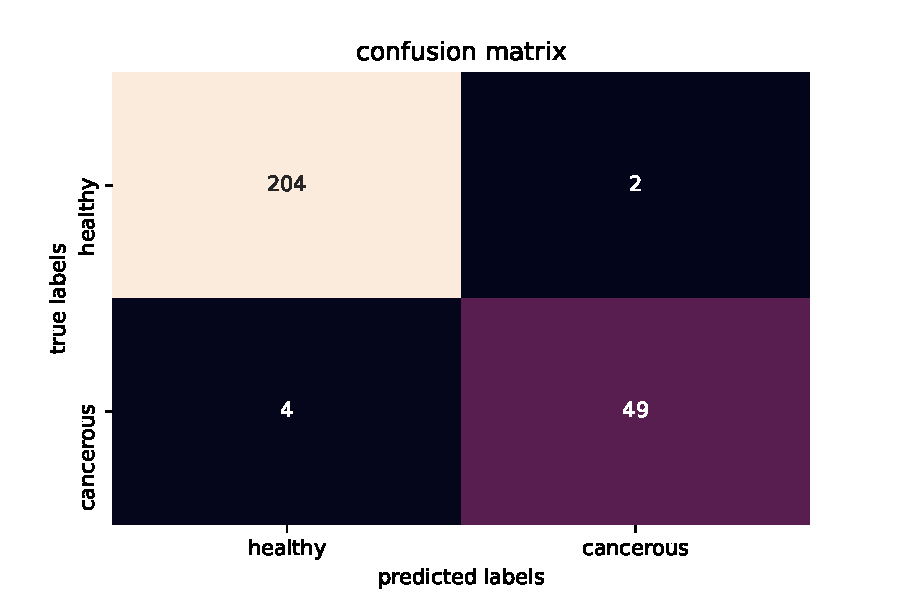
\includegraphics[width=90mm]{imagenes/confusion_mat3_gpflow}
	\caption{Matriz de confusión para Fold 3 kernel radial}
	\label{fig:conf3}
\end{figure}

\begin{table}[H]
	\centering
	\begin{tabular}{lllll}
		\textbf{acc} & \textbf{precision} & \textbf{specificity} & \textbf{recall} & \textbf{f1-score} \\
		0.976834     & 0.960784           & 0.990291             & 0.924528        & 0.942308         \\
	\end{tabular}
	\caption{Resultados obtenidos Fold 3 kernel radial}
	\label{table:3}
\end{table}

Este tercer modelo, al igual que los anteriores obtiene buenos resultados, valores en las curvas casi perfectos, valores bastante altos en todas las métricas que se han calculado, etc... La diferencia entre este modelo y el anterior es que este obtiene un peor valor para el \textit{Recall} y por lo tanto sí que ha clasificado imágenes de tejido canceroso como tejido sano y es peor modelo que el modelo anterior.

\subsubsection{Fold 4}

\begin{figure}[H]
	\centering
	\subfigure{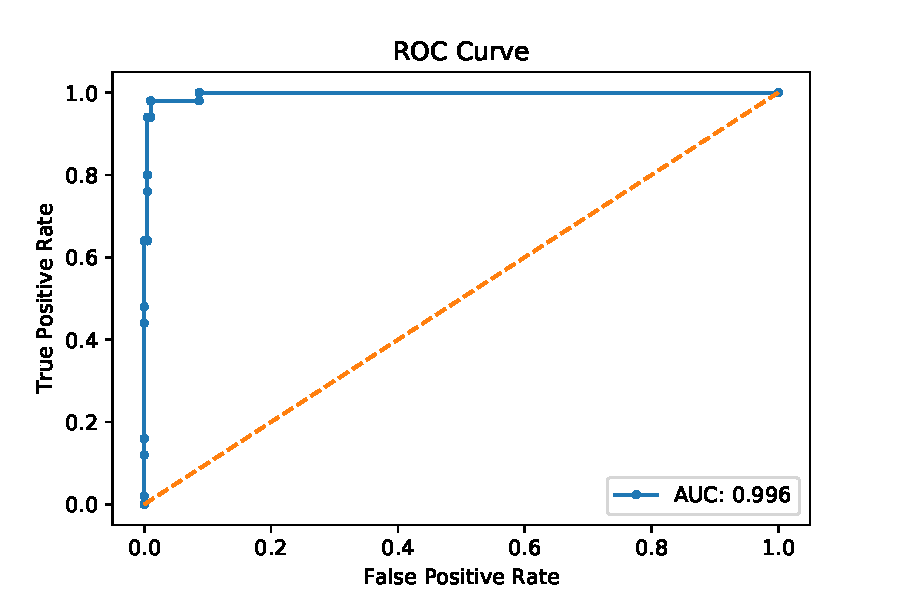
\includegraphics[width=60mm]{imagenes/p4_roc_gpflow}}
	\subfigure{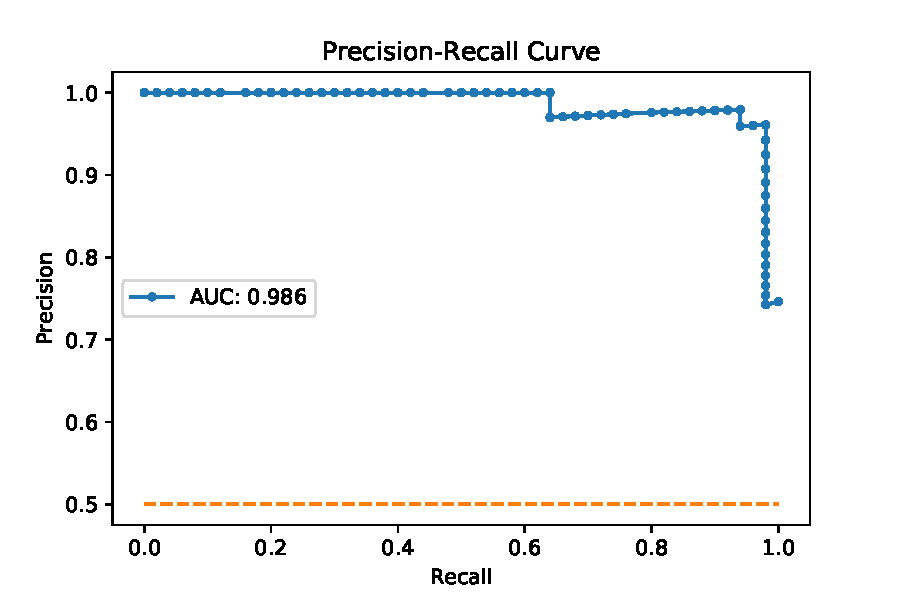
\includegraphics[width=60mm]{imagenes/p4_curve_gpflow}}
	\caption{Curva Roc y Curva Precision-Recall Fold 4 kernel radial}
	\label{fig:resultados4}
\end{figure}

\begin{figure}[H]
	\centering
	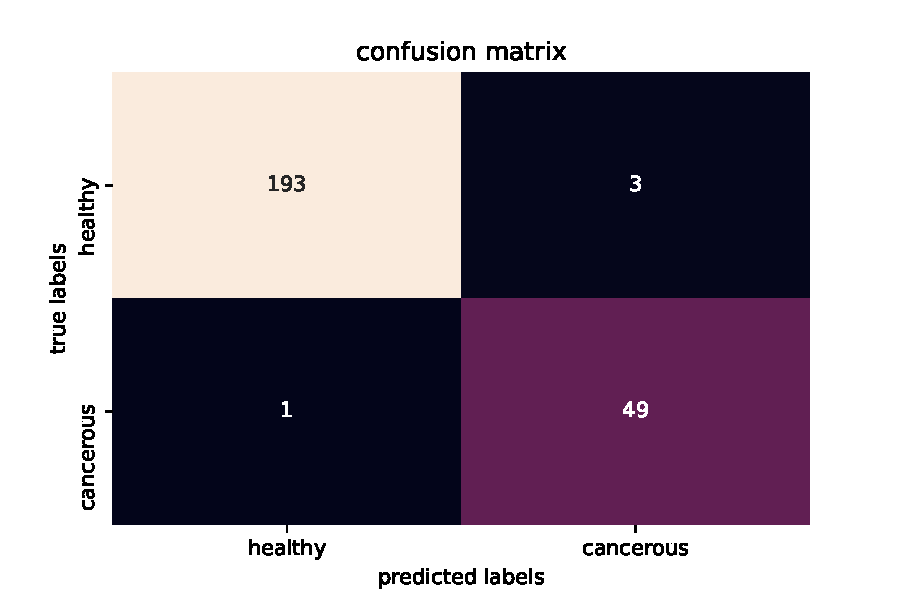
\includegraphics[width=90mm]{imagenes/confusion_mat4_gpflow}
	\caption{Matriz de confusión para Fold 4 kernel radial}
	\label{fig:conf4}
\end{figure}

\begin{table}[H]
	\centering
	\begin{tabular}{lllll}
		\textbf{acc} & \textbf{precision} & \textbf{specificity} & \textbf{recall} & \textbf{f1-score} \\
		0.983740     & 0.942308           & 0.984694             & 0.980000        & 0.960784         \\
	\end{tabular}
	\caption{Resultados obtenidos Fold 4 kernel radial}
	\label{table:4}
\end{table}

De este modelo se puede destacar su curva de \textit{Precision-Recall}, aunque el valor de \textit{AUC} sea bastante bueno, se pude ver que al final la precisión desciende bastante a diferencia del resto modelo. Si nos fijamos en la matriz de confusión se puede ver que el número de \textit{Falsos Negativos} es menor que el número de \textit{Falsos Positivos}; de ahí que el valor de \textit{Recall} sea mayor que el valor de \textit{Precision}.

\subsubsection{Fold 5}

\begin{figure}[H]
	\centering
	\subfigure{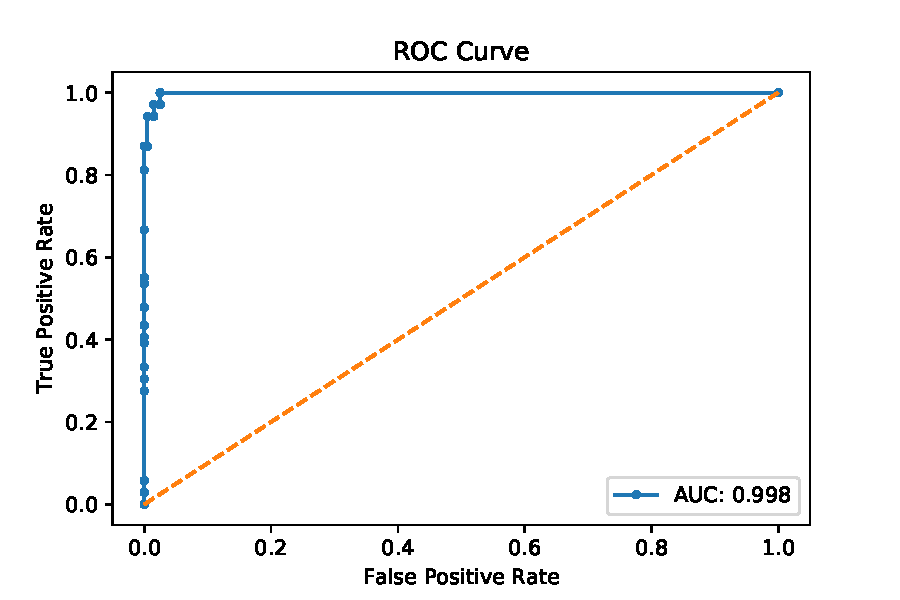
\includegraphics[width=60mm]{imagenes/p5_roc_gpflow}}
	\subfigure{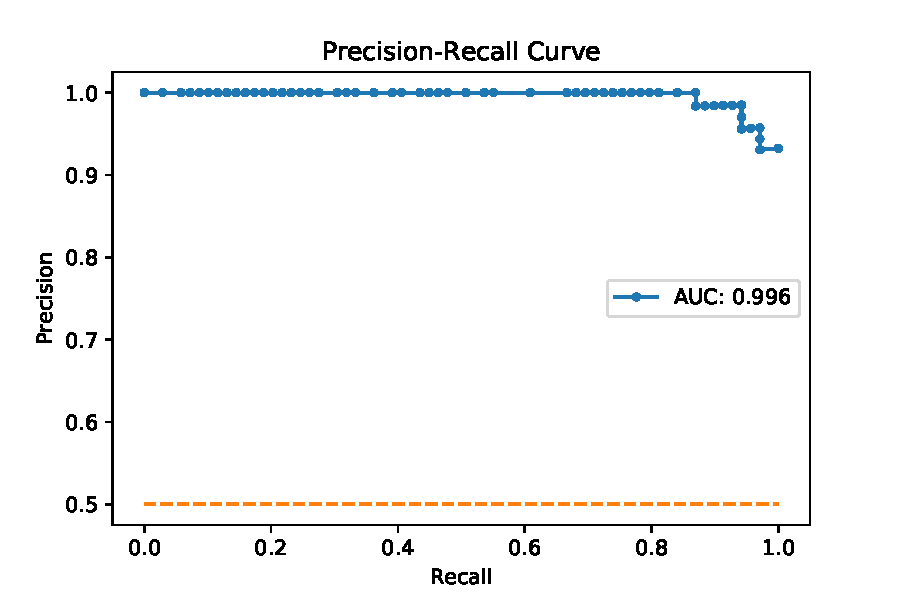
\includegraphics[width=60mm]{imagenes/p5_curve_gpflow}}
	\caption{Curva Roc y Curva Precision-Recall Fold 5 kernel radial}
	\label{fig:resultados5}
\end{figure}

\begin{figure}[H]
	\centering
	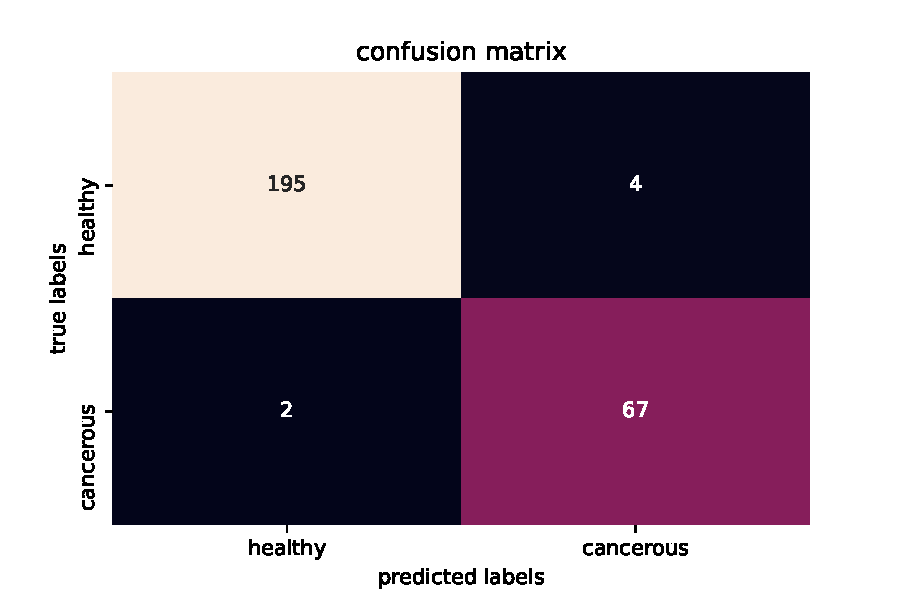
\includegraphics[width=90mm]{imagenes/confusion_mat5_gpflow}
	\caption{Matriz de confusión para Fold 5 kernel radial}
	\label{fig:conf5}
\end{figure}

\begin{table}[H]
	\centering
	\begin{tabular}{lllll}
		\textbf{acc} & \textbf{precision} & \textbf{specificity} & \textbf{recall} & \textbf{f1-score} \\
		0.977612     & 0.943662           & 0.979899             & 0.971014        & 0.957143        
	\end{tabular}
	\caption{Resultados obtenidos Fold 5 kernel radial}
	\label{table:5}
\end{table}

Para este último modelo se pueden ver resultados parecidos al resto de modelos en la métricas, buenos valores en las curvas; manteniendo un buen equilibrio entre \textit{Precision} y \textit{Recall}; obteniendo un número de \textit{Falsos Negativos} menor que \textit{Falsos Positivos}.

\subsection{Núcleo Lineal}
\subsubsection{Fold 1}

\begin{figure}[H]
	\centering
	\subfigure{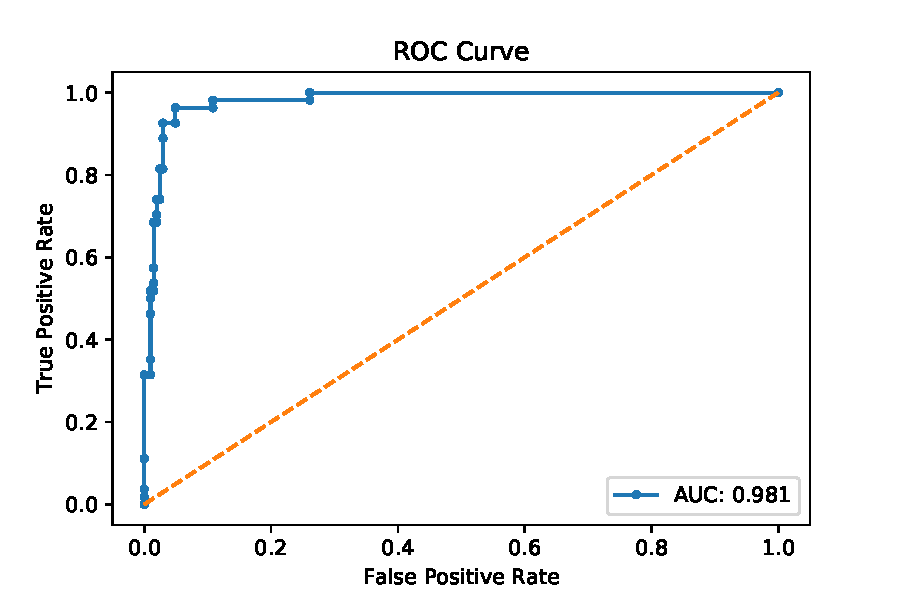
\includegraphics[width=60mm]{imagenes/p1_roc_gpflow_linear}}
	\subfigure{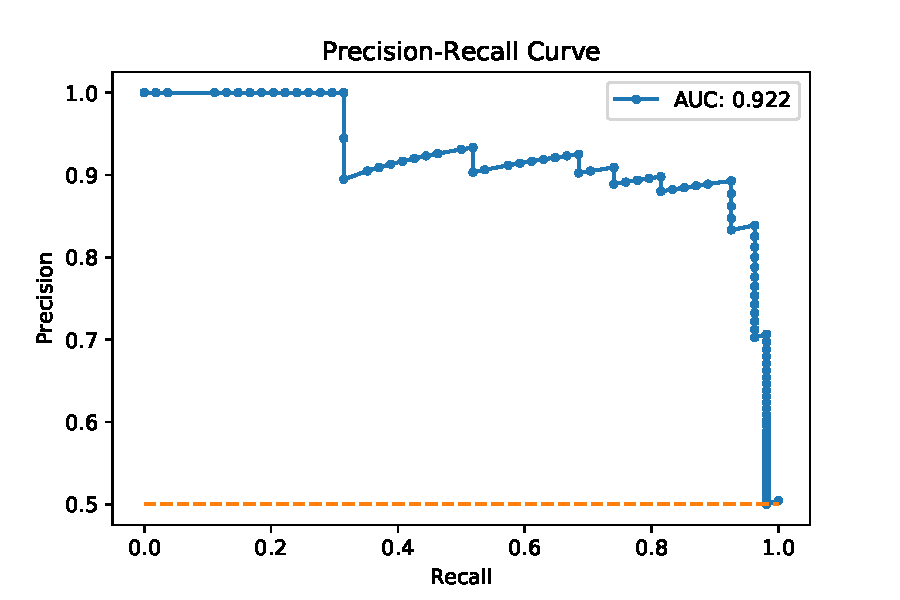
\includegraphics[width=60mm]{imagenes/p1_curve_gpflow_linear}}
	\caption{Curva Roc y Curva Precision-Recall Fold 1 kernel lineal}
	\label{fig:resultados1_linear}
\end{figure}

\begin{figure}[H]
	\centering
	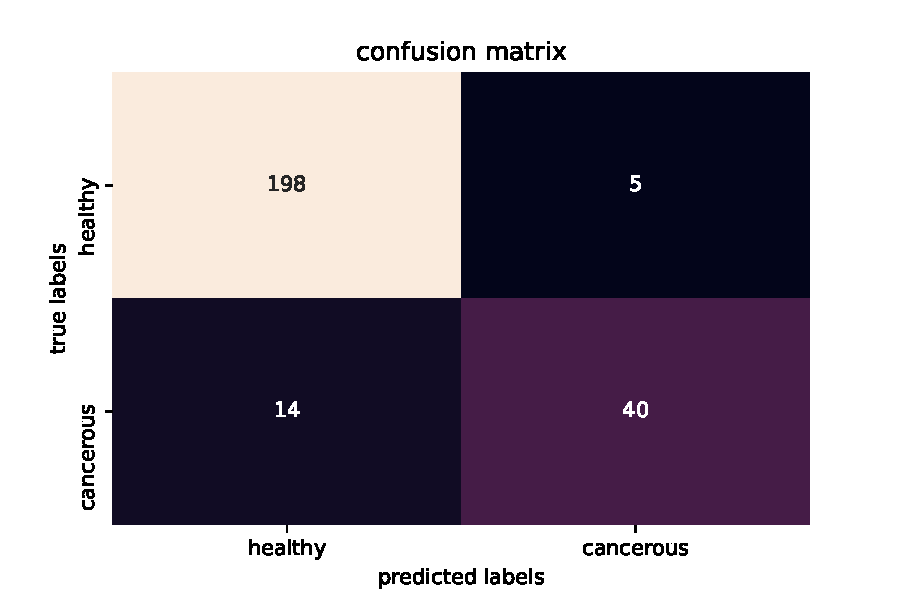
\includegraphics[width=90mm]{imagenes/confusion_mat1_gpflow_linear}
	\caption{Matriz de confusión para Fold 1 kernel lineal}
	\label{fig:conf1_lin}
\end{figure}

\begin{table}[H]
	\centering
	\begin{tabular}{lllll}
		\textbf{acc} & \textbf{precision} & \textbf{specificity} & \textbf{recall} & \textbf{f1-score} \\
		0.926070     & 0.888889           & 0.975369             & 0.740741        & 0.808081         \\
	\end{tabular}
	\caption{Resultados obtenidos Fold 1 kernel lineal}
	\label{table:6}
\end{table}

Para este primer modelo podemos ver valores bastante buenos en los \textit{AUC} de las curvas, estando ambos por encima del 90\%; se puede destacar la \textit{curva Precision-Recall} que desciende bastante. Si nos fijamos en la matriz de confusión o en las medidas obtenidas se puede ver un número de \textit{Falsos Negativos} mucho mayor que el de \textit{Falsos Positivos}, esto también se refleja en los valores de \textit{Precision} y \textit{Recall} y explica la forma de la \textit{curva Precision-Recall}.

\subsubsection{Fold 2}

\begin{figure}[H]
	\centering
	\subfigure{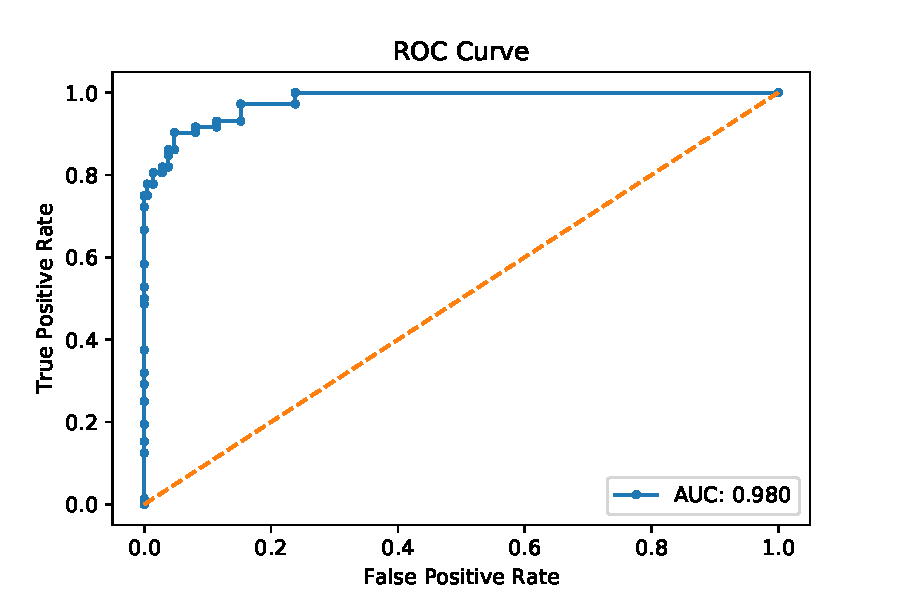
\includegraphics[width=60mm]{imagenes/p2_roc_gpflow_linear}}
	\subfigure{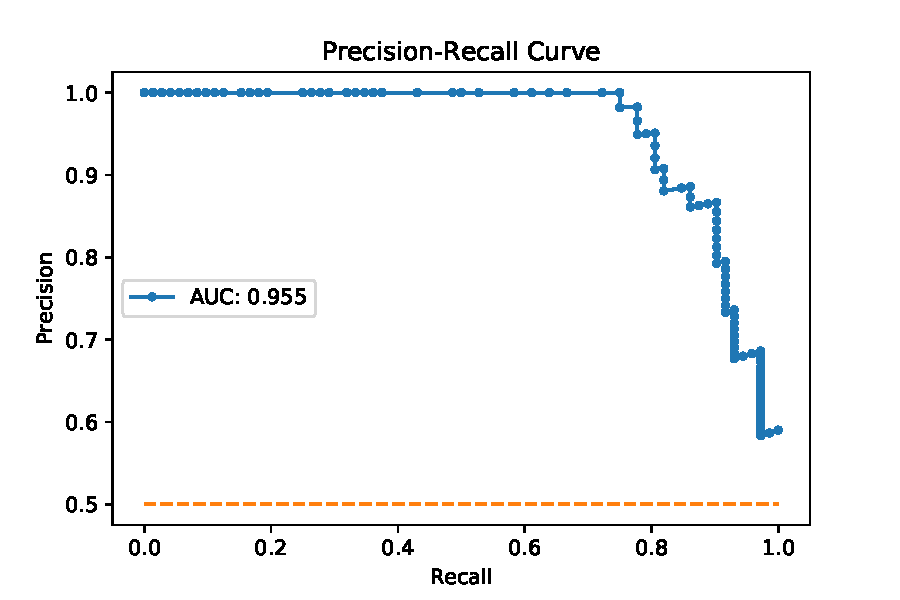
\includegraphics[width=60mm]{imagenes/p2_curve_gpflow_linear}}
	\caption{Curva Roc y Curva Precision-Recall Fold 2 kernel lineal}
	\label{fig:resultados2_linear}
\end{figure}

\begin{figure}[H]
	\centering
	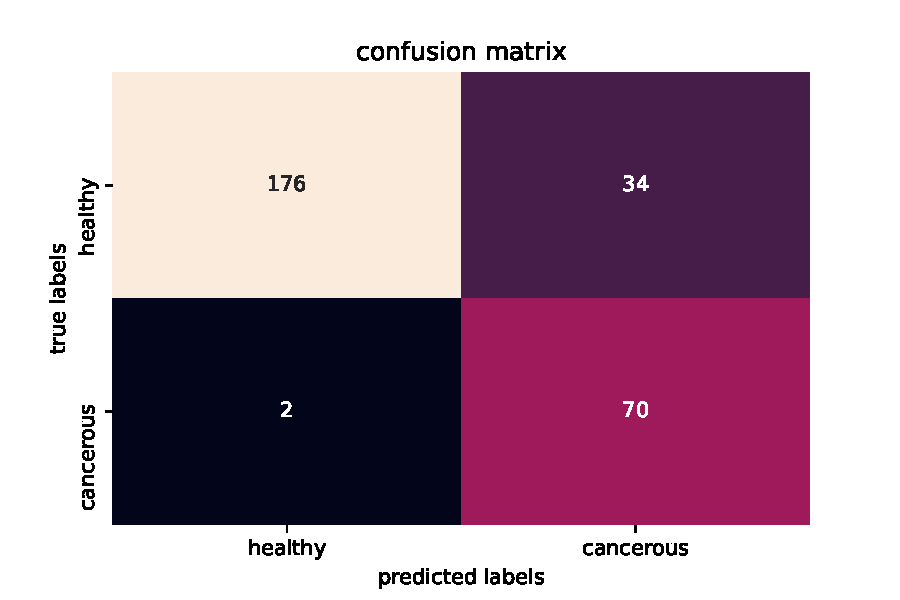
\includegraphics[width=90mm]{imagenes/confusion_mat2_gpflow_linear}
	\caption{Matriz de confusión para Fold 2 kernel lineal}
	\label{fig:conf2_lin}
\end{figure}

\begin{table}[H]
	\centering
	\begin{tabular}{lllll}
		\textbf{acc} & \textbf{precision} & \textbf{specificity} & \textbf{recall} & \textbf{f1-score} \\
		0.872340     & 0.673077           & 0.838095             & 0.972222        & 0.795455         \\
	\end{tabular}
	\caption{Resultados obtenidos Fold 2 kernel lineal}
	\label{table:7}
\end{table}

Para este segundo modelo podemos ver resultados justamente contrarios a los del modelo anterior, el número de \textit{Falsos Positivos} es mucho mayor que el de \textit{Falsos Negativos}. Por ello este modelo no es bueno ya que no es capaz de diferenciar entre tejido sano y tejido canceroso, aunque es mejor que el modelo anterior porque se equivoca normalmente clasificando imágenes sanas como cancerosas y no al revés.

\subsubsection{Fold 3}

\begin{figure}[H]
	\centering
	\subfigure{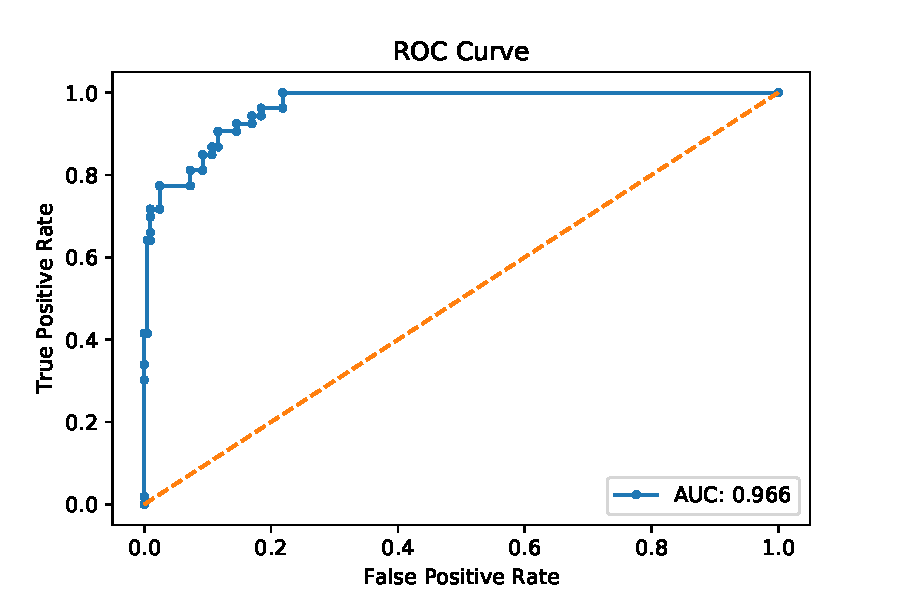
\includegraphics[width=60mm]{imagenes/p3_roc_gpflow_linear}}
	\subfigure{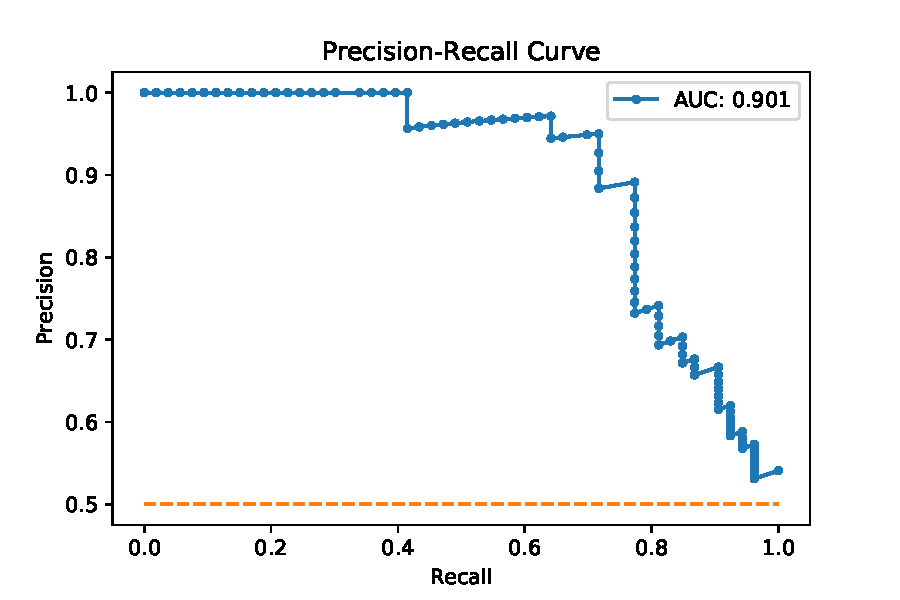
\includegraphics[width=60mm]{imagenes/p3_curve_gpflow_linear}}
	\caption{Curva Roc y Curva Precision-Recall Fold 3 kernel lineal}
	\label{fig:resultados3_linear}
\end{figure}

\begin{figure}[H]
	\centering
	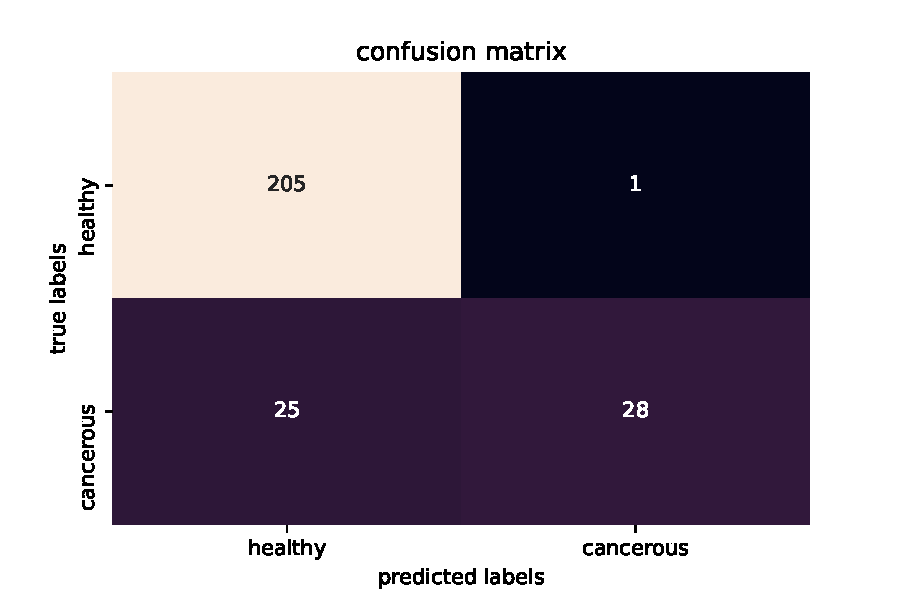
\includegraphics[width=90mm]{imagenes/confusion_mat3_gpflow_linear}
	\caption{Matriz de confusión para Fold 3 kernel lineal}
	\label{fig:conf3_lin}
\end{figure}

\begin{table}[H]
	\centering
	\begin{tabular}{lllll}
		\textbf{acc} & \textbf{precision} & \textbf{specificity} & \textbf{recall} & \textbf{f1-score} \\
		0.899614     & 0.965517           & 0.995146             & 0.528302        & 0.682927         \\      
	\end{tabular}
	\caption{Resultados obtenidos Fold 3 kernel lineal}
	\label{table:8}
\end{table}

Este modelo también es bastante malo, ya que aunque los valores de \textit{Accuracy} o \textit{AUC} es las curvas calculadas no sean malos, su valor de \textit{Recall} es demasiado bajo y por ello el valor de \textit{F1-score} también; por lo tanto este modelo no sería interesante para predecir.

\subsubsection{Fold 4}

\begin{figure}[H]
	\centering
	\subfigure{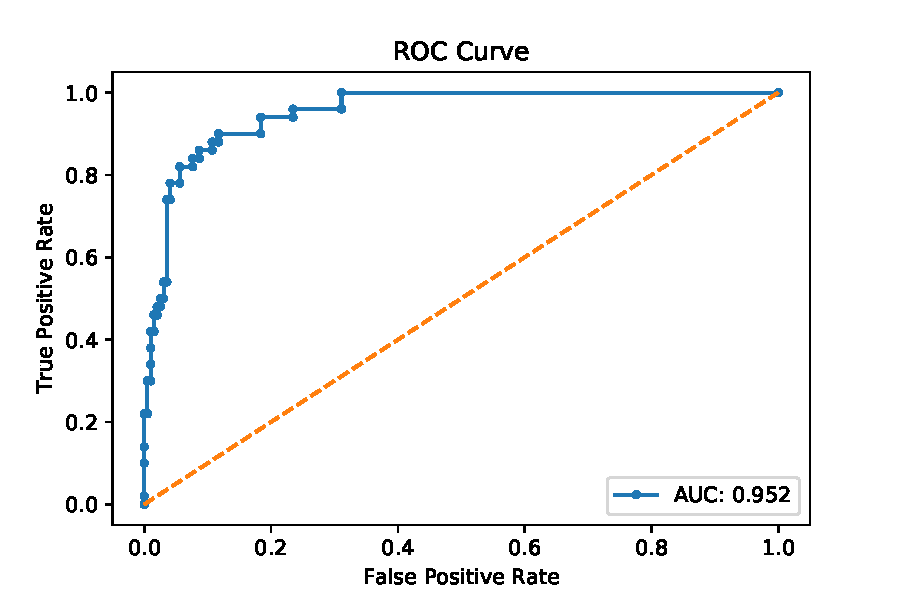
\includegraphics[width=60mm]{imagenes/p4_roc_gpflow_linear}}
	\subfigure{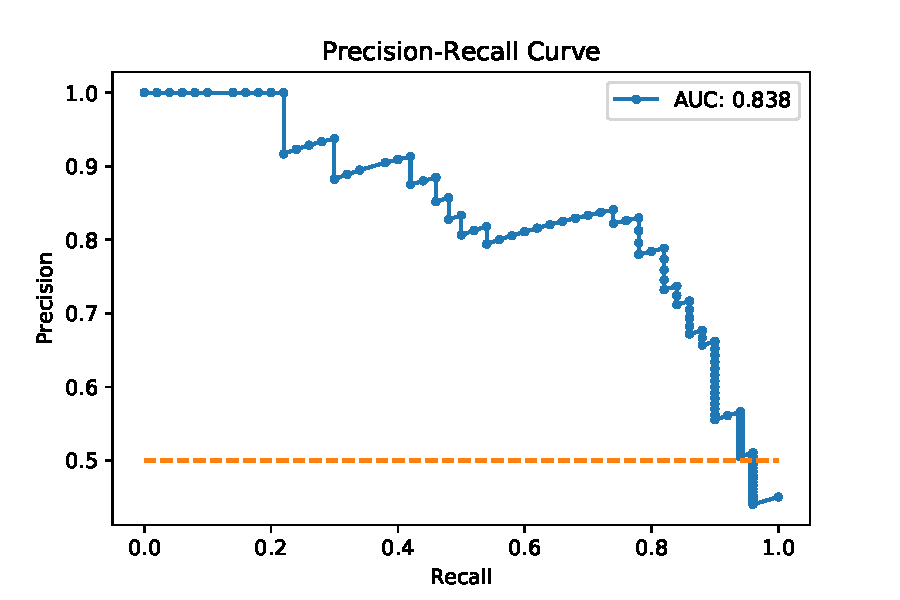
\includegraphics[width=60mm]{imagenes/p4_curve_gpflow_linear}}
	\caption{Curva Roc y Curva Precision-Recall Fold 4 kernel lineal}
	\label{fig:resultados4_linear}
\end{figure}

\begin{figure}[H]
	\centering
	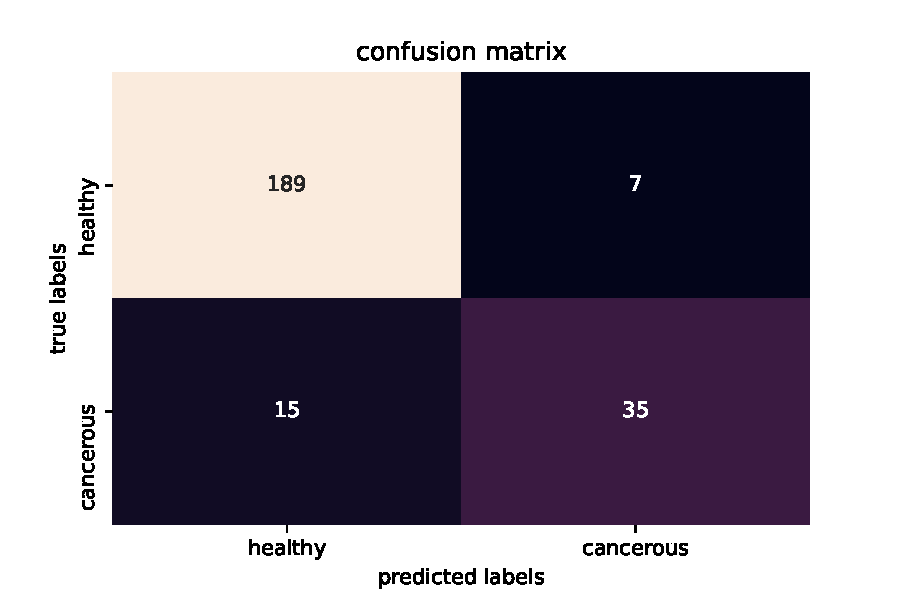
\includegraphics[width=90mm]{imagenes/confusion_mat4_gpflow_linear}
	\caption{Matriz de confusión para Fold 4 kernel lineal}
	\label{fig:conf4_lin}
\end{figure}

\begin{table}[H]
	\centering
	\begin{tabular}{lllll}
		\textbf{acc} & \textbf{precision} & \textbf{specificity} & \textbf{recall} & \textbf{f1-score} \\
		0.910569     & 0.833333           & 0.964286             & 0.700000        & 0.760870         \\
	\end{tabular}
	\caption{Resultados obtenidos Fold 4 kernel lineal}
	\label{table:9}
\end{table}

De este modelo se puede destacar el valor de \textit{AUC} de la \textit{curva Precision-Recall}, siendo este el más bajo obtenido. Aunque los valores obtenidos no sean demasiado malos y no destaque por equivocarse demasiado al clasificar cualquiera de las clases, no es igual de bueno que el modelo generado con el kernel radial para este mismo conjunto de datos.
\subsubsection{Fold 5}

\begin{figure}[H]
	\centering
	\subfigure{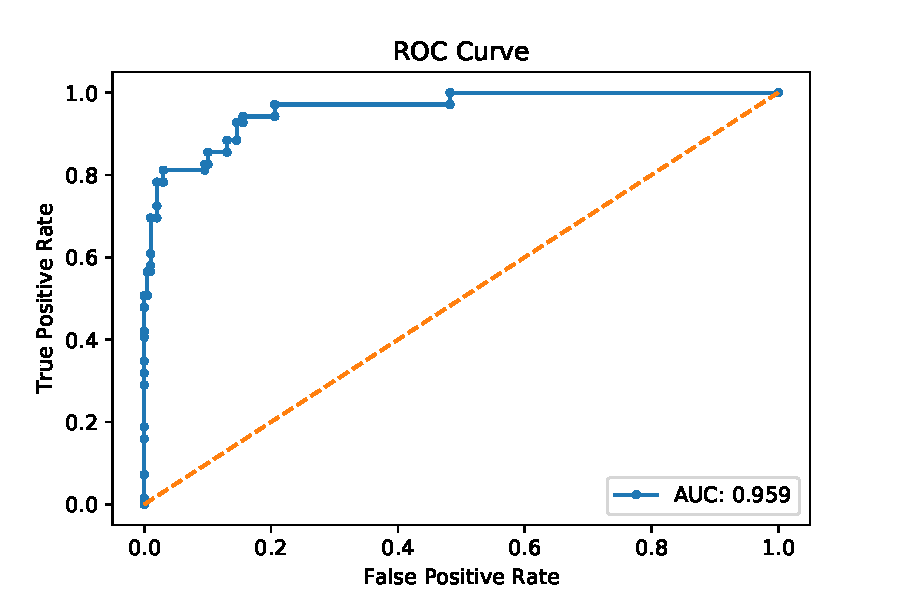
\includegraphics[width=60mm]{imagenes/p5_roc_gpflow_linear}}
	\subfigure{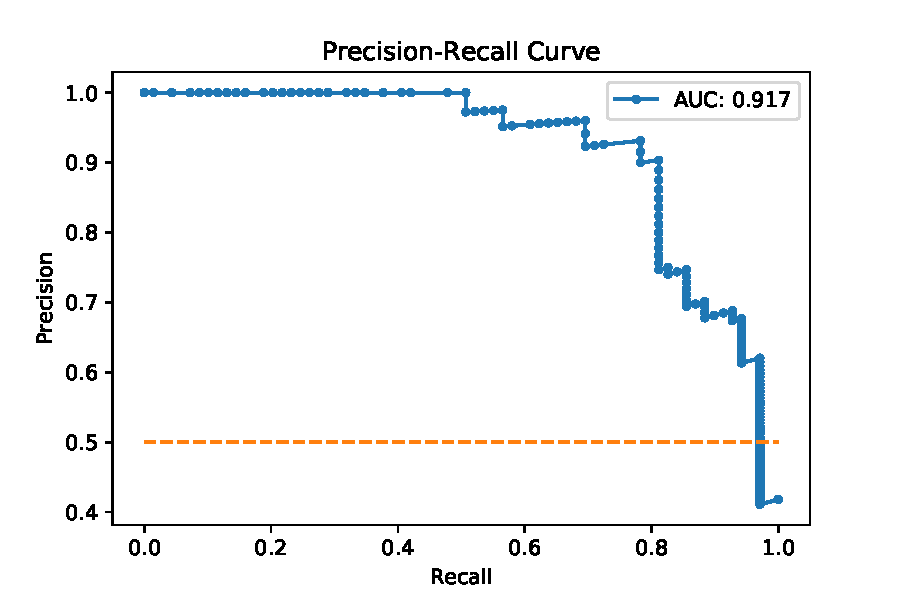
\includegraphics[width=60mm]{imagenes/p5_curve_gpflow_linear}}
	\caption{Curva Roc y Curva Precision-Recall Fold 5 kernel lineal}
	\label{fig:resultados5_linear}
\end{figure}

\begin{figure}[H]
	\centering
	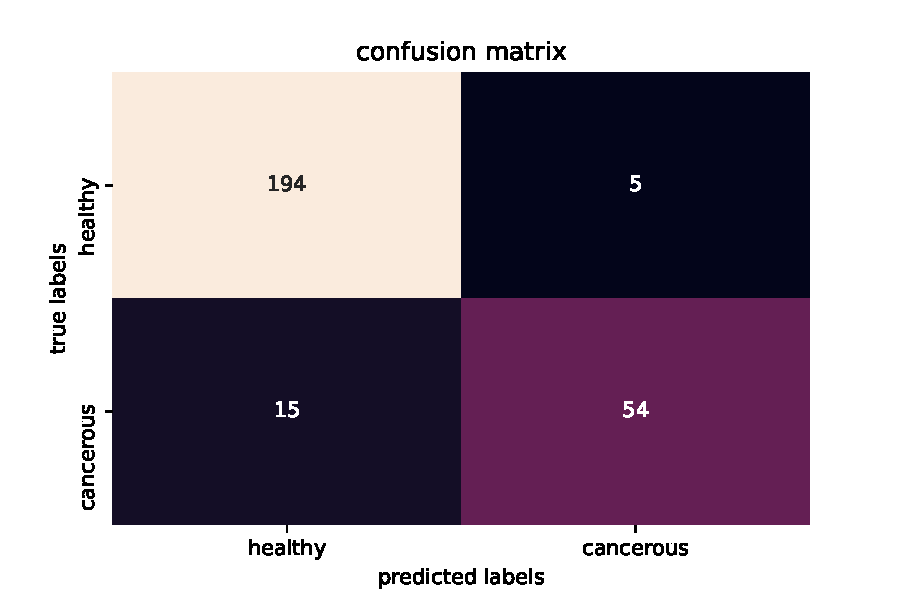
\includegraphics[width=90mm]{imagenes/confusion_mat5_gpflow_linear}
	\caption{Matriz de confusión para Fold 5 kernel lineal}
	\label{fig:conf5_lin}
\end{figure}

\begin{table}[H]
	\centering
	\begin{tabular}{lllll}
		\textbf{acc} & \textbf{precision} & \textbf{specificity} & \textbf{recall} & \textbf{f1-score} \\
		0.925373     & 0.915254           & 0.974874             & 0.782609        & 0.843750        
	\end{tabular}
	\caption{Resultados obtenidos Fold 5 kernel lineal}
	\label{table:10}
\end{table}

Este modelo obtiene relativamente buenos resultados; el valor de \textit{Recall} es algo bajo y esto se refleja también en la matriz de confusión. Al igual que el resto de modelos, la \textit{curva Precision-Recall} disminuye mucho conforme el valor de \textit{Recall} aumenta.

\section{Clasificación de nuevos datos}
Si se quisiera clasificar nuevos datos, bastaría con utilizar el modelo seleccionado y hacer predicción sobre este nuevo dato con dicho modelo. Para ello, sería necesario guardar el modelo ya entrenado para no tener que repetir el proceso de training. Una vez obtenida la predicción, si sabemos cual es la clase real de dicho nuevo dato; o hay un experto que pueda saber la clase real de dicho dato, se puede comprobar si la predicción del modelo es correcta. Si el modelo que se ha entrenado ha encontrado realmente las características importantes que diferencian las clases la predicción de este modelo debería de ser correcta. Si se prueban nuevos datos y las predicciones son erróneas; se debe volver entrenar el modelo añadiendo dichos nuevos datos; ya que es posible que los datos que se hayan utilizado para generar el modelo no represente todo el espacio de ejemplos que puede haber para ese clasificador.\newline

Para el caso que se estudia en esta práctica, se utilizaría el segundo modelo entrenado con kernel radial. Antes de realizar la predicción, se debe particionar las imágenes en bloques de 2048x2048 y se calculan sus descriptores LBP uniforme invariante y se generan los histogramas; una vez hecho esto se puede utilizar el clasificador para predecir la clase de dicho bloque. Una vez se ha obtenido la predicción, si se dispone de un anatomopatólogo se le debería de preguntar si dicha predicción es correcta.

\section{Experimentos adicional}
Para aumentar el número de datos que tenemos en el modelo, se podría utilizar algún método de oversamplig, por ejemplo \textit{BLSMOTE}. \textit{BLSMOTE} es una modificación del algoritmo \textit{SMOTE}, dicho algoritmo genera nuevas instancias a partir de la combinación de dos instancias de los datos; dichas instancias son un dato aleatorio del dataset y otro dato cercano al primero. La diferencia entre \textit{SMOTE} y \textit{BLSMOTE} es que este último solamente selecciona datos que se encuentran en la periferia entre una clase y otra.\newline

Utilizar este método puede ser interesante por lo que se ha observado durante los experimentos realizados, con los modelos de kernel lineal se obtenían modelos peores que con los modelos con kernel radial. Gracias a esto podemos saber que los datos no son linealmente separables o existen algunas partes en las que los datos de clases diferentes están entremezclados y por ello se la frontera entre un dato y otro no está bien definida. Dado esto, al generar nuevos datos solamente por la periferia de la clase minoritaria podemos mejorar el ajuste del modelo con los datos.\newline

Una vez hecho oversampling sobre el conjunto de los datos solamente se construiría un conjunto de train y otro de test; con el conjunto de train se entería un único modelo de Proceso Gaussiano. Tras esto se comprobaría la calidad del modelo obtenido haciendo la predicción con los datos de test y se obtendrían las diferentes métricas.
